\chapter{Introduction}
Le projet réalisé s'inscrit dans le cadre d’une démarche d’approfondissement des notions abordées en cours de programmation générative. Ce projet propose, dans sa première partie, l'étude et l’implémentation de deux cas concrets :
\begin{itemize}
   \item Les tas binaires
   \item Les B-arbres
\end{itemize}

À partir de cette première étape, nous avons, dans une deuxième partie, porté notre analyse sur l'étude d'une hiérarchie plus complète pouvant englober les deux cas concrets cités précédemment ainsi que d'autres implémentations d'arborescences comme les tas binaires, tas binomiaux, B-arbre, arbre rouge-noir etc...

Le but de la démarche de ce projet est d'aboutir sur des programmes robustes et fiables en mettant en oeuvre les principes vus en cours et en TD à savoir la généricité, l'utilisation des templates ainsi qu'une gestion rigoureuse de la mémoire.
\begin{figure}[h]
	\centering
%	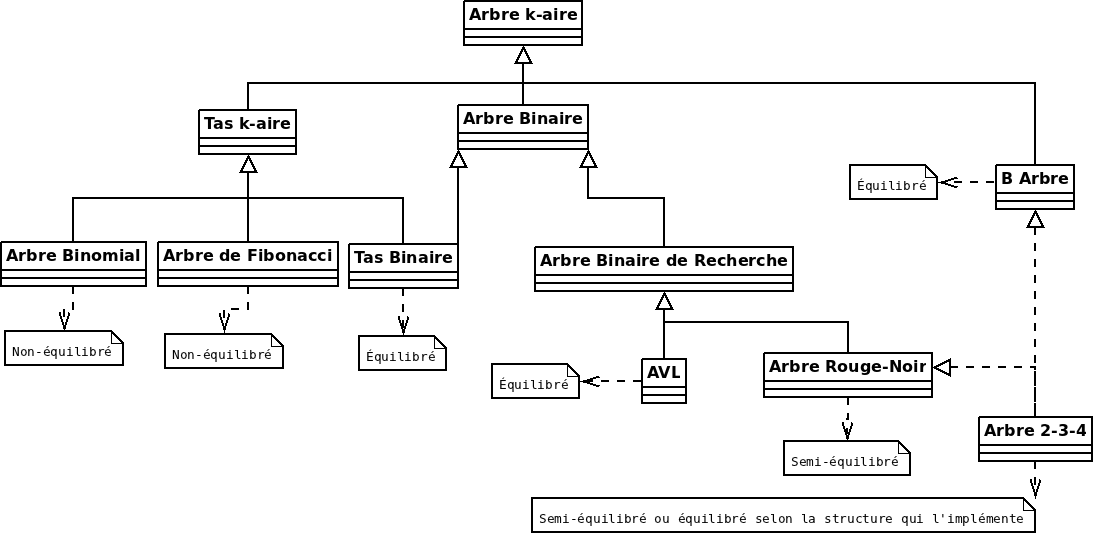
\includegraphics[scale=0.5]{Hierarchie_arbres}
	\caption{Une hiérarchie sur les arbres}
	\label{fig:hierarchie}
\end{figure}
Le but de la démarche de ce projet est d'aboutir sur des programmes robustes et fiables en mettant en oeuvre les principes vus en cours et en TD à savoir la généricité, l'utilisation des templates ainsi qu'une gestion rigoureuse de la mémoire.
